% Welcome to KernTeX!
%
% This project is a short tour of what LaTeX can do. Every section shows the
% source next to the result -- change anything, press Ctrl+S and watch the PDF
% on the right update. You can't break anything: reopen this project any time
% via the command palette (Ctrl+K) -> "Open example project".
\documentclass[11pt,a4paper]{article}

% --- Fonts & encoding (pdfLaTeX needs fontenc; XeTeX/Tectonic is Unicode) ---
\usepackage{iftex}
\ifPDFTeX
  \usepackage[T1]{fontenc}
  \usepackage{lmodern}
\fi
\usepackage[margin=2.5cm]{geometry}
\usepackage{microtype}

% --- Packages used in this tour ---
\usepackage{amsmath, amssymb}   % mathematics
\usepackage{graphicx}           % \includegraphics
\usepackage{booktabs}           % nice tables
\usepackage{xcolor}             % colours
\usepackage{tikz}               % drawings
\usepackage{listings}           % code listings
\usepackage[backend=bibtex, style=numeric]{biblatex}
\addbibresource{references.bib}
\usepackage[colorlinks, linkcolor=blue!60!black, urlcolor=blue!60!black, citecolor=green!40!black]{hyperref}

\lstset{basicstyle=\ttfamily\small, columns=fullflexible, frame=single,
  keywordstyle=\color{blue!70!black}\bfseries, commentstyle=\color{gray}}

\newcommand{\source}[1]{\par\noindent\textcolor{gray}{\small\texttt{#1}}\par\medskip}

\title{Welcome to \textsf{KernTeX}}
\author{A short tour of \LaTeX}
\date{\today}

\begin{document}
\maketitle

\begin{abstract}
  This document is your playground. It shows the most common things you will
  do in \LaTeX{}: structure, formatting, lists, mathematics, tables, figures,
  cross-references, a bibliography, drawings and code. Each section is short ---
  read the source in the editor on the left side by side with this PDF.
\end{abstract}

\tableofcontents

\section{Structure}
\label{sec:structure}
Documents are split with \verb|\section|, \verb|\subsection| and
\verb|\subsubsection|. The table of contents above is generated automatically.

\subsection{A subsection}
Paragraphs are separated by an empty line in the source.

Like this one. Line breaks inside a paragraph are ignored, so you can wrap
your source however you like.

\section{Formatting}
You can write \textbf{bold}, \textit{italic}, \underline{underlined},
\texttt{typewriter}, \textsc{Small Caps} and \textcolor{blue!70!black}{coloured}
text. Sizes range from {\small small} to {\large large} and {\Large larger}.
Quotes are written ``like this'', dashes as en--dash and em---dash.

\section{Lists}
\begin{itemize}
  \item Bullet points with \verb|itemize|
  \item can be
  \begin{enumerate}
    \item nested and
    \item numbered with \verb|enumerate|.
  \end{enumerate}
\end{itemize}
\begin{description}
  \item[Description lists] pair a term with an explanation.
\end{description}

\section{Mathematics}
\label{sec:math}
Inline math goes between dollar signs: $a^2 + b^2 = c^2$. Displayed equations
get a number you can refer to:
\begin{equation}
  \int_{-\infty}^{\infty} e^{-x^2}\,\mathrm{d}x = \sqrt{\pi}
  \label{eq:gauss}
\end{equation}
Several aligned lines use \verb|align|:
\begin{align}
  f(x) &= (x + 1)^2 \\
       &= x^2 + 2x + 1
\end{align}
Matrices and other structures:
\[
  A = \begin{pmatrix} 1 & 2 \\ 3 & 4 \end{pmatrix}, \qquad
  \sum_{k=1}^{n} k = \frac{n(n+1)}{2}, \qquad
  \forall \varepsilon > 0 \; \exists \delta > 0
\]

\section{Tables}
Table~\ref{tab:engines} uses the \verb|booktabs| package for clean rules.
\begin{table}[htbp]
  \centering
  \begin{tabular}{lll}
    \toprule
    Engine   & Unicode & Comes with \\
    \midrule
    Tectonic & yes     & KernTeX (built in) \\
    pdfLaTeX & limited & TeX Live, MiKTeX \\
    XeLaTeX  & yes     & TeX Live, MiKTeX \\
    LuaLaTeX & yes     & TeX Live, MiKTeX \\
    \bottomrule
  \end{tabular}
  \caption{TeX engines you can choose in KernTeX's settings.}
  \label{tab:engines}
\end{table}

\section{Figures}
Images are included with \verb|\includegraphics| (PNG, JPG and PDF work).
Figure~\ref{fig:example} lives in the \texttt{images} folder of this project.
\begin{figure}[htbp]
  \centering
  
\includegraphics[width=0.45\textwidth]{images/example.png}
  \caption{An example image.}
  \label{fig:example}
\end{figure}

\section{Cross-references}
Give anything a \verb|\label{...}| and refer to it with \verb|\ref{...}|,
\verb|\eqref{...}| or \verb|\pageref{...}|: Section~\ref{sec:math} contains
Equation~\eqref{eq:gauss} on page~\pageref{eq:gauss}. In the editor, type
\verb|\ref{| and KernTeX suggests all labels of the project.

\section{Bibliography}
Sources live in \texttt{references.bib}. Cite them with \verb|\cite|:
\LaTeX{} was created by Lamport~\cite{lamport1994}, building on Knuth's
\TeX~\cite{knuth1984}. Typing \verb|\cite{| suggests all keys.
Tips on writing are in~\cite{strunk}.

\section{Drawings with TikZ}
\begin{center}
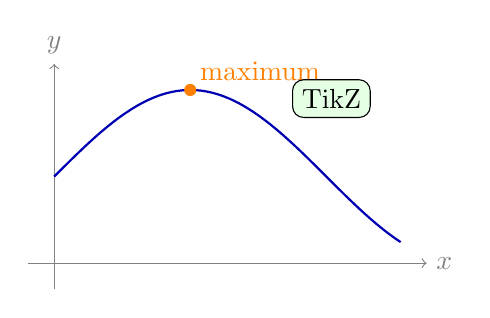
\begin{tikzpicture}[scale=1.1]
  \draw[->, gray] (-0.3,0) -- (4.3,0) node[right] {$x$};
  \draw[->, gray] (0,-0.3) -- (0,2.3) node[above] {$y$};
  \draw[thick, blue!70!black, domain=0:4, samples=60] plot (\x, {1 + sin(\x r)});
  \fill[orange] (1.5708, 2) circle (2pt) node[above right] {maximum};
  \node[draw, rounded corners, fill=green!10] at (3.2,1.9) {TikZ};
\end{tikzpicture}
\end{center}

\section{Code listings}
\begin{lstlisting}[language=Python]
def greet(name):
    # Comments are grey, keywords blue.
    return f"Hello, {name}!"
\end{lstlisting}

\section{Footnotes and links}
Footnotes are numbered automatically.\footnote{Like this one.} Links work too:
\url{https://www.ctan.org} or \href{https://github.com/nicolasasauer/kerntex}{KernTeX on GitHub}.

\section{KernTeX tips}
\begin{description}
  \item[Ctrl+S] Save and compile (can be turned off in Settings).
  \item[Ctrl+K] Command palette --- every action, searchable.
  \item[Ctrl+F] Find and replace in the current file.
  \item[Ctrl+Space] Autocompletion for commands, labels and citations.
  \item[Problems panel] Click an error to jump to its line.
  \item[File tree] Right-click a file to rename it, move it to the trash or
    make it the main file.
\end{description}
New projects can start from templates (article, thesis, presentation, letter).
Projects are ordinary folders --- you can use them with Git, Overleaf or any
other editor.

\printbibliography

\end{document}
